\documentclass[a4paper, 12pt, twocolumn]{article}
\usepackage[utf8]{inputenc}
% \DeclareUnicodeCharacter{2217}{*}
\usepackage{apacite}
\usepackage{hyperref}
\usepackage{amsmath, graphicx}
\usepackage{lipsum}
\usepackage{abstract}
\usepackage[a4paper, margin=1in]{geometry}
\usepackage{hyperref}
\usepackage{setspace}
\usepackage{mathptmx} %times new roman font in pdfLaTeX
\usepackage{amsfonts}
\usepackage{times}
\usepackage{xcolor}
\usepackage{fancyhdr}
\usepackage{natbib}
\usepackage{tabularx}
\usepackage{multicol}
\usepackage{multirow}
\usepackage{adjustbox}
\usepackage{caption}
\usepackage{authblk}

\usepackage{fontspec}
\setmainfont{Times New Roman} 

\title{Characterization of Atmospheric Pressure Circular Dielectric Barrier Discharge via lectrical and Optical Methods}

\author[1, *]{\href{https://dev.jsdhami.com.np}{Janak Singh Dhami}}
\author[1, 2]{Manish Pandey}
\author[3]{Abhinav Thakur}


\affil[1]{\textit{Department of Physics, Tri-Chandra Multiple Campus, Kathmandu, Nepal}}
\affil[2]{\textit{Department of Physics, St. Xaiver's College, Maitighar, Kathmandu, Nepal}}
\affil[3]{\textit{Department of Physics, Patan Multiple Campus, Lalitpur Nepal}}
\date{}
\pagestyle{fancy}

\lhead{}
\chead{\textit{Janak S. Dhami et al./ BIBECHANA 21 (2024) 195-212}}
\rhead{\thepage}

% footer
\cfoot{}
\lfoot{}
\rfoot{}


\begin{document}
\twocolumn[
\begin{@twocolumnfalse}
\maketitle 
\onehalfspacing

\begin{center}
    \text{*Corresponding author Email: \href{mailto:janak.795401@trc.tu.edu.np}{janak.795401@trc.tu.edu.np}}
\end{center}

\begin{abstract}
\noindent 
This research examines electrical and optical properties of atmospheric pressure circular dielectric barrier discharge (APCDBD) in natural air. Airflow and input voltage effects on power consumption are studied. The discharge energy and power per cycle are derived from Lissajous plots and voltage-current curves. Light emissions during plasma discharge determine electron excitation, rotational, and vibrational temperatures, and plasma density. The Boltzmann plot technique estimates electron excitation temperature, while MassiveOES software calculates rotational and vibrational temperatures. Results show increased filamentary microdischarges with rising airflow and voltage. \\

\noindent
\textbf{\textit{Keywords: Plasma Physics, Research, Template, Research, Workshop \\ \\}} 
\end{abstract}

\end{@twocolumnfalse}
]

\section{Introduction}
\noindent
orem ipsum dolor sit amet, consectetuer adi-
piscing elit. Ut purus elit, vestibulum ut, place-
rat ac, adipiscing vitae, felis \cite{Dahal2024}. Curabitur dictum
gravida mauris. Nam arcu libero, nonummy
eget, consectetuer id, vulputate a, magna. Do-
nec vehicula augue eu neque. Pellentesque ha-
bitant morbi tristique senectus et netus et ma-
lesuada fames ac turpis egestas. Mauris ut leo.
Cras viverra metus rhoncus sem. Nulla et lec-
tus vestibulum urna fringilla ultrices. Phasel-
lus eu tellus sit amet tortor gravida placerat.
Integer sapien est, iaculis in, pretium quis, vi-
verra ac, nunc. Praesent eget sem vel leo ul-
trices bibendum. Aenean faucibus. Morbi do-
lor nulla, malesuada eu, pulvinar at, mollis ac,
nulla. Curabitur auctor semper nulla \cite{Dahal2024}. Donec
varius orci eget risus. Duis nibh mi, congue eu,
accumsan eleifend, sagittis quis, diam. Duis
eget orci sit amet orci dignissim rutrum \cite{Hao2024}.
\lipsum[1-1]

\subsection{Background}
\lipsum[1-1]

\section{Materials and Methods}
\lipsum[2-2]

\begin{table}[h]
    \centering
    \caption{Details of Students}
    \renewcommand{\arraystretch}{1.5}
    \begin{tabular}{|c|c|c|}
    \hline
       S.N.  & Name of Student & Addr.\\ \hline
       1  & Janak S. Dhami & KTM\\ \hline
       2  & Janak S. Dhami & KTM\\ \hline
       3  & Janak S. Dhami & KTM\\ \hline
    \end{tabular}
    \label{tab:my_label}
\end{table}

\lipsum[2-2]
\\
\begin{figure}
    \centering
    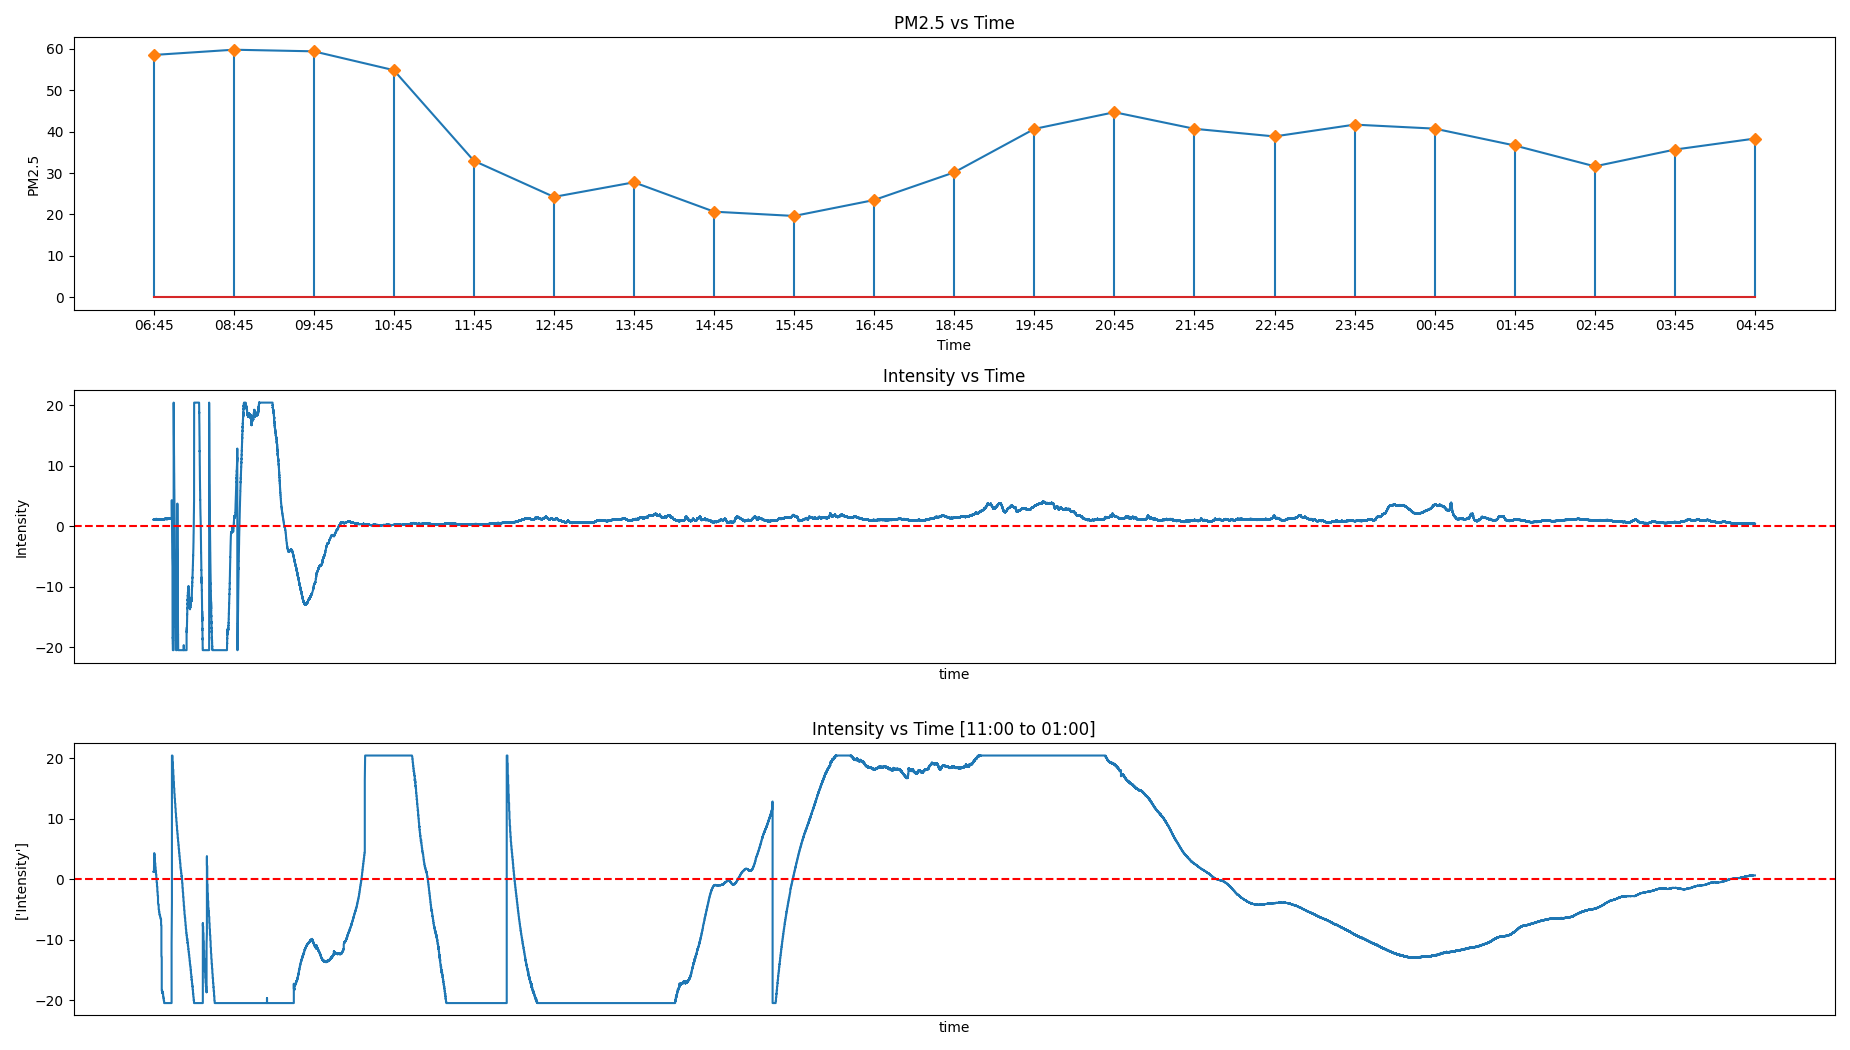
\includegraphics[width=1\linewidth]{images/aq.png}
    \caption{Air Quality in KTM}
    \label{aq}
\end{figure}

\lipsum[1-1]
\begin{enumerate}
    \item The integral $\int_0^1 x^{m-1}(1-x)^{n-1}dx, (m>0, n>0)$ is known as first integral or $\beta$-function.
    \item the integral ....
    \item \[(a+b)^2\]
    \item 
\end{enumerate}


\section{Results}
\lipsum[2-2]
\\
$E = mc^2$ this is main formula of albert.

\begin{equation}
    x = \frac{-b\pm \sqrt{b^2-4ac}}{2a}
\end{equation}

\section{Conclusion}
\lipsum[1-2]

\begin{figure}[ht]
    \centering
    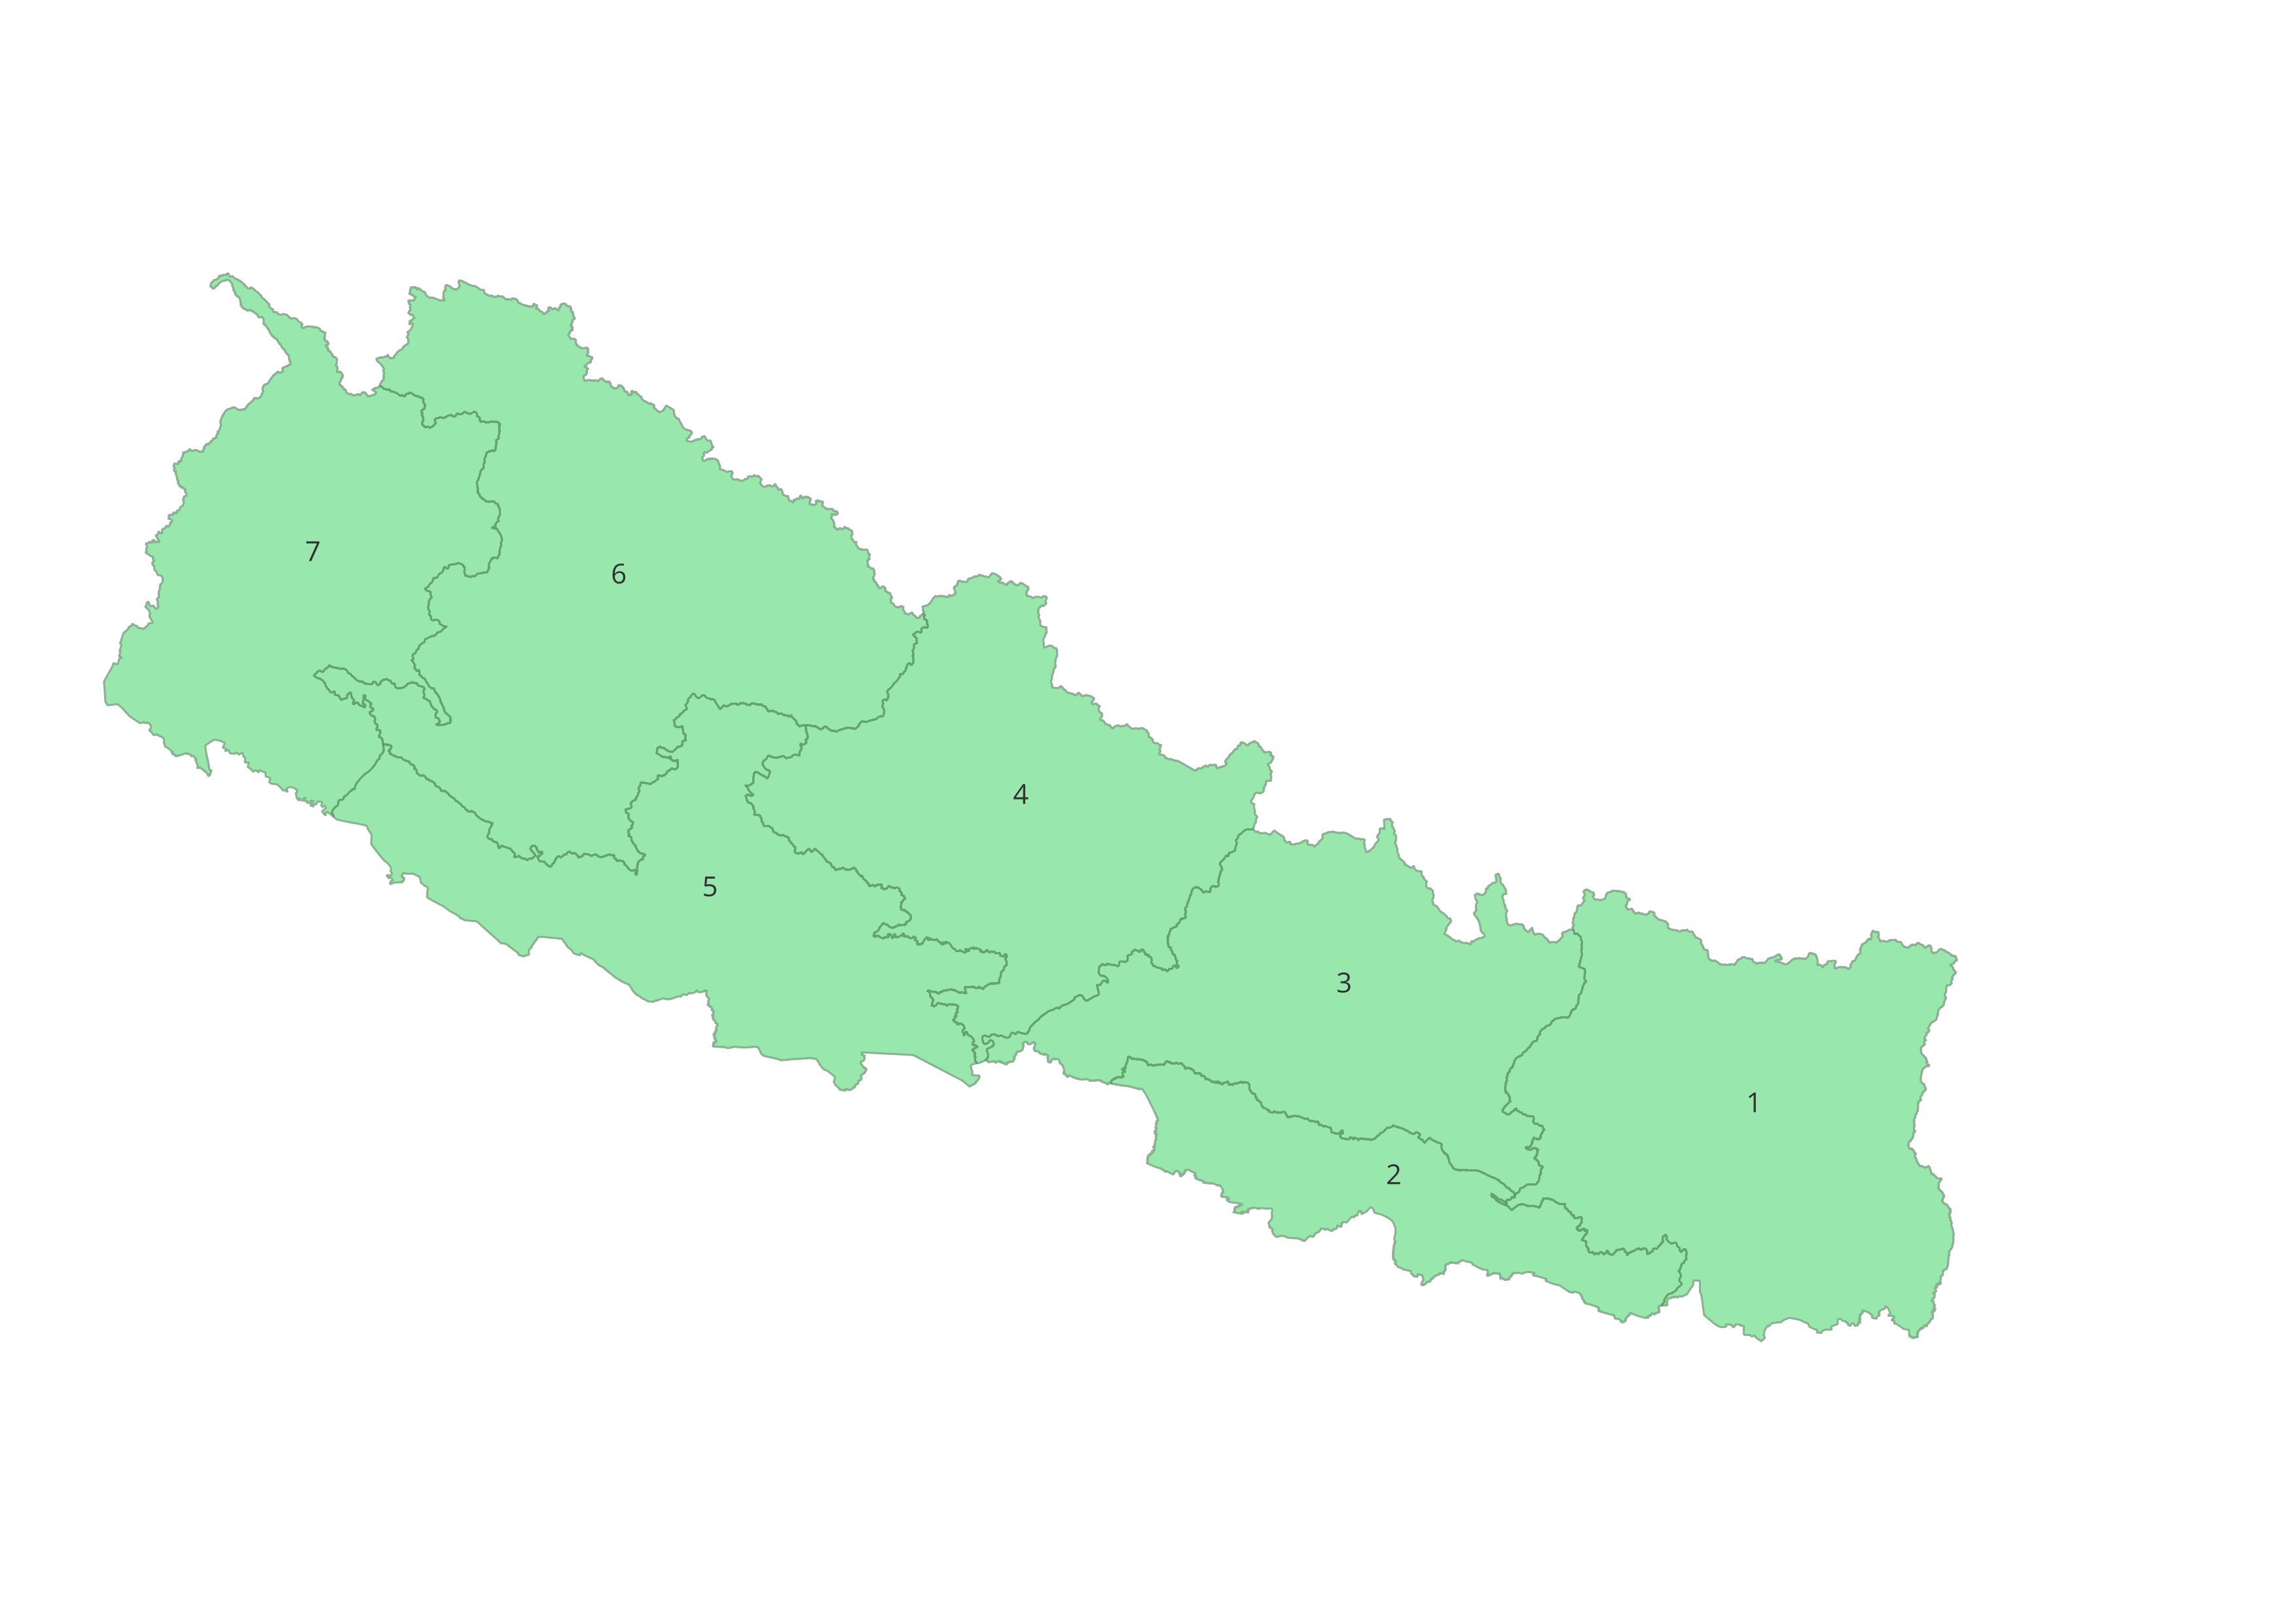
\includegraphics[width=1\linewidth]{images/np.png}
    \caption{Map of Nepal}
    \label{national map}
\end{figure}


\begin{figure}
    \centering
    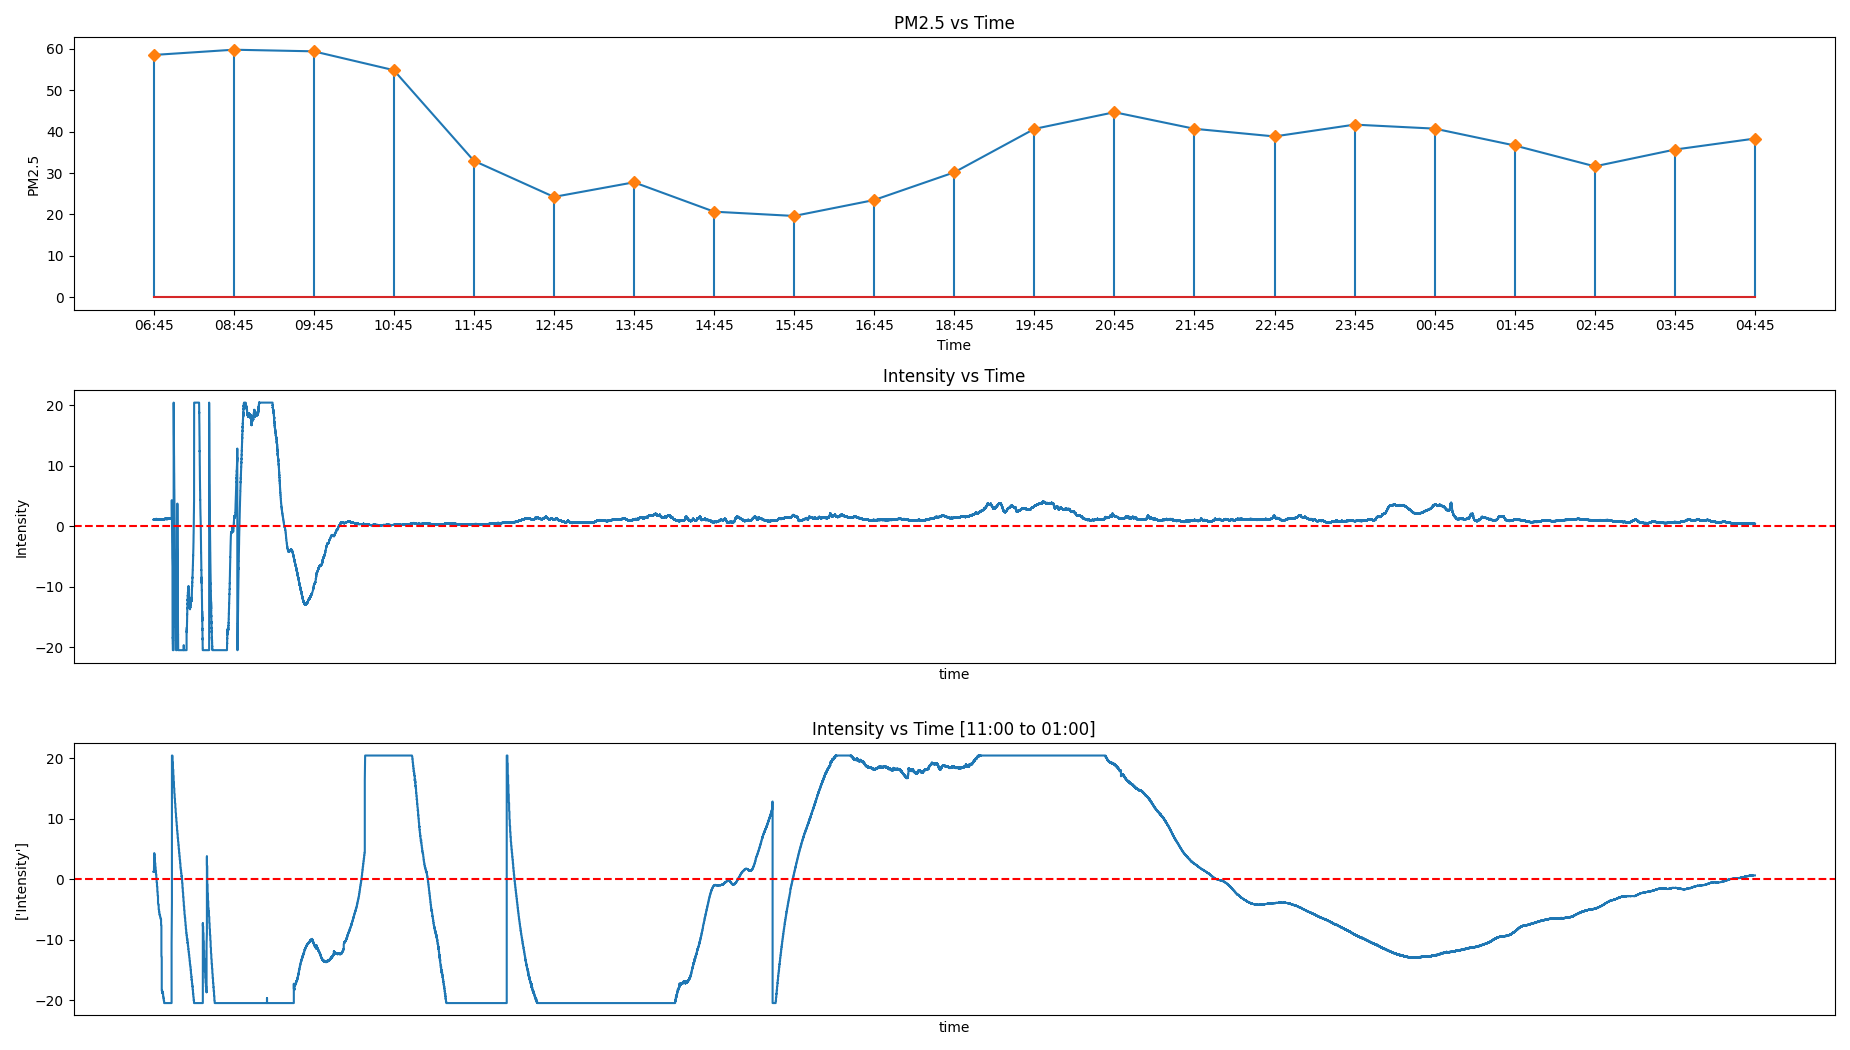
\includegraphics[width=1\linewidth]{images/aq.png}
    \caption{Nepali Map}
    \label{fig:enter-label}
\end{figure}
\lipsum[2-3]


% single column in twocolumn page
\twocolumn[
    \begin{@twocolumnfalse}
        \bibliographystyle{apacite}
        \bibliography{references}
    \end{@twocolumnfalse}
]

\end{document}
